\documentclass[../notes.tex]{subfiles}

\pagestyle{main}
\renewcommand{\chaptermark}[1]{\markboth{\chaptername\ \thechapter\ (#1)}{}}
\stepcounter{chapter}

\begin{document}




\chapter{Introduction to Representation Theory}
\section{Matrix Representations of Symmetry Operations}
\begin{itemize}
    \item \marginnote{10/3:}Tools for identifying symmetry elements.
    \begin{itemize}
        \item Chem 3D (visualization).
        \item \href{https://symotter.org/gallery}{Otterbein University symmetry gallery} (examples of molecules that satisfy all of the point groups).
    \end{itemize}
    \item Gives examples of molecules that satisfy the high-symmetry point groups.
    \begin{itemize}
        \item $C_{\infty v}$: \ce{CO}.
        \item $D_{\infty h}$: \ce{CO2}.
        \item $T_d$: \ce{CH4}.
        \item $T_h$: \ce{[Co(NO2)6]^3+}.
        \begin{itemize}
            \item $T_h$ is $T_d$ with $\sigma_h$ symmetry.
        \end{itemize}
        \item $O_h$: \ce{[Co(NH3)6]^3+}
        \item $I_h$: N/a.
        \begin{itemize}
            \item 120 symmetry elements in total; we will not be asked to identify all of these!
        \end{itemize}
        \item $K_h$: N/a.
        \begin{itemize}
            \item Symmetry of the sphere.
        \end{itemize}
        \item $T,O,I$ are subgroups of $T_h,O_h,I_h$, respectively, and only have proper (not improper) rotations. These are very rare point groups. An example of a molecule in the $T$ point group is \ce{[Ca(THF)6]^2+}.
    \end{itemize}
    \item Learn $T,O,I$ from Otterbein University example and ask questions!
    \item Low symmetry: $C_1,C_i,C_s$.
    \item The mirror plane in a $C_s$ molecule is denoted by $\sigma$ (no subscript).
    \item \textbf{Vector}: A series of numbers which we write in a row or a column.
    \item \textbf{Matrix}: Any rectangular array of numbers set between two brackets.
    \item Basics of matrix multiplication: $A\cdot\vec{x}=\vec{y}$ given in terms of matrix multiplication, e.g., if $A$ is $n\times m$ and $\vec{x}\in\R^m$, then
    \begin{equation*}
        y_i = \sum_{j=1}^ma_{ij}x_j
    \end{equation*}
    for $i=1,\dots,n$.
    \item Matrix representations:
    \begin{itemize}
        \item $E$: What matrix $A$ satisfies $A\cdot\vec{x}=\vec{x}$ for all $\vec{x}$? The $3\times 3$ matrix $I$ does.
        \item $i$: What matrix $A$ satisfies $A\cdot\vec{x}=-\vec{x}$ for all $\vec{x}$? The $3\times 3$ matrix $-I$ does.
        \item $\sigma_{xy}$: What matrix $A$ flips the sign of the $z$-coordinate of $\vec{x}$? The $3\times 3$ matrix $\diag(1,1,-1)$ does.
        \item $C_2$: What matrix $A$ flips the sign of the $x,y$-coordinates of $\vec{x}$? The $3\times 3$ matrix $\diag(-1,-1,1)$ does.
        \item $C_3$: Consider a $C_{3v}$ molecule.
        \begin{figure}[H]
            \centering
            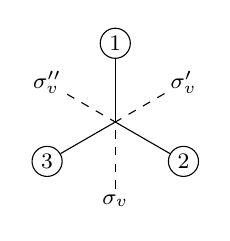
\begin{tikzpicture}
                \footnotesize
                \node [circle,draw,inner sep=1.5pt] at (90:1) {1}
                    edge (0,0)
                ;
                \node [circle,draw,inner sep=1.5pt] at (-30:1) {2}
                    edge (0,0)
                ;
                \node [circle,draw,inner sep=1.5pt] at (-150:1) {3}
                    edge (0,0)
                ;
        
                \node [inner sep=2pt] at (-90:1) {$\sigma_v$}
                    edge [dashed] (0,0)
                ;
                \node [inner sep=2pt] at (30:1) {$\sigma_v'$}
                    edge [dashed] (0,0)
                ;
                \node [inner sep=2pt] at (150:1) {$\sigma_v''$}
                    edge [dashed] (0,0)
                ;
            \end{tikzpicture}
            \caption{$C_3$ matrix representation setup.}
            \label{fig:C3MatrixSetup}
        \end{figure}
        Instead of describing a rotation in $\R^3$ using radians, we can think of a rotation as a permutation of the numbered atoms. So in this example,
        \begin{equation*}
            \underbrace{
                \begin{bmatrix}
                    0 & 1 & 0\\
                    0 & 0 & 1\\
                    1 & 0 & 0\\
                \end{bmatrix}
            }_{C_3}
            \begin{bmatrix}
                1\\
                2\\
                3\\
            \end{bmatrix}
            =
            \begin{bmatrix}
                2\\
                3\\
                1\\
            \end{bmatrix}
        \end{equation*}
    \end{itemize}
    \item We will only be asked for matrix representations of very simple things, e.g., these or \ang{90} or \ang{180} turns.
    \item The above matrices form a mathematical group, which obeys the same multiplication table as the operations.
    \begin{itemize}
        \item For example,
        \begin{equation*}
            \underbrace{
                \begin{bmatrix}
                    -1 & 0 & 0\\
                    0 & -1 & 0\\
                    0 & 0 & 1\\
                \end{bmatrix}
            }_{C_2}
            \underbrace{
                \begin{bmatrix}
                    1 & 0 & 0\\
                    0 & 1 & 0\\
                    0 & 0 & -1\\
                \end{bmatrix}
            }_{\sigma_h}
            =
            \underbrace{
                \begin{bmatrix}
                    -1 & 0 & 0\\
                    0 & -1 & 0\\
                    0 & 0 & -1\\
                \end{bmatrix}
            }_i
        \end{equation*}
    \end{itemize}
    \item The matrix representations given above are not the "simplest" way of describing these symmetry operations.
    \begin{itemize}
        \item The simplest way is using the \textbf{character}.
        \item We find the character using a \textbf{similarity transformation} to take our matrix representations to block-diagonalized forms and then compute the characters of the blocks from there.
        \item Recall that analogous blocks multiply in a block-diagonal matrix.
    \end{itemize}
    \item \textbf{Character} (of a symmetry operation): The trace (sum of the diagonal elements) of the matrix representation of that operation. \emph{Denoted by} $\bm{\chi}$.
    \item \textbf{Similarity transformation} (matrix): The matrix which, when conjugated with a matrix representation of a symmetry operation, yields the block-diagonalized form of that matrix. \emph{Denoted by} $\bm{R}$.
    \begin{itemize}
        \item We don't need to know how to compute these.
    \end{itemize}
    \item Similarity transformation example: The $C_3$ matrix representation given above is not block diagonal, but there exists a matrix $R$ (that we don't have to know how to find) such that
    \begin{equation*}
        RC_3R^{-1} =
        \begin{bNiceArray}{c|cc}[margin]
            1 & 0 & 0\\
            \hline
            0 & -\frac{1}{2} & \frac{\sqrt{3}}{2}\\
            0 & -\frac{\sqrt{3}}{2} & -\frac{1}{2}
        \end{bNiceArray}
    \end{equation*}
    \begin{itemize}
        \item The characters of the blocks of the above matrix are 1 and $-1$, respectively. The character of the overall matrix is still 0.
    \end{itemize}
\end{itemize}



\section{Characters and Irreducible Representations}
\begin{itemize}
    \item \marginnote{10/5:}The PSet has been posted --- remember that its graded for completion.
    \begin{itemize}
        \item Answer key will be posted the day it's due.
        \item Submit via email or give her a printed copy/write it out on blank paper (preferred).
    \end{itemize}
    \item Review: \ce{NH3} is in the $C_{3v}$ point group.
    \item Denote the bond vectors of \ce{NH3} by $d_1,d_2,d_3$. Let's use them as a basis of the representation $\Gamma$. Also label the hydrogen atoms 1-3.
    \begin{table}[h!]
        \centering
        \small
        \tabulinesep=1mm
        \begin{tabu}{|p{2cm}|l|l|}
            \hline
            \textbf{Symmetry element} & \textbf{Matrix} & \textbf{Character}\\
            \hline
            $E$ & $
                \begin{bmatrix}
                    1 & 0 & 0\\
                    0 & 1 & 0\\
                    0 & 0 & 1\\
                \end{bmatrix}
                \begin{bmatrix}
                    H_1\\
                    H_2\\
                    H_3\\
                \end{bmatrix}
                =
                \begin{bmatrix}
                    H_1\\
                    H_2\\
                    H_3\\
                \end{bmatrix}
            $ & 3\\
            \hline
            $C_3$ & $
                \begin{bmatrix}
                    0 & 1 & 0\\
                    0 & 0 & 1\\
                    1 & 0 & 0\\
                \end{bmatrix}
                \begin{bmatrix}
                    H_1\\
                    H_2\\
                    H_3\\
                \end{bmatrix}
                =
                \begin{bmatrix}
                    H_2\\
                    H_3\\
                    H_1\\
                \end{bmatrix}
            $ & 0\\
            \hline
            ${C_3}^2$ & $
                \begin{bmatrix}
                    0 & 0 & 1\\
                    1 & 0 & 0\\
                    0 & 1 & 0\\
                \end{bmatrix}
                \begin{bmatrix}
                    H_1\\
                    H_2\\
                    H_3\\
                \end{bmatrix}
                =
                \begin{bmatrix}
                    H_3\\
                    H_1\\
                    H_2\\
                \end{bmatrix}
            $ & 0\\
            \hline
            $\sigma_v$ (along $d_1$) & $
                \begin{bmatrix}
                    1 & 0 & 0\\
                    0 & 0 & 1\\
                    0 & 1 & 0\\
                \end{bmatrix}
                \begin{bmatrix}
                    H_1\\
                    H_2\\
                    H_3\\
                \end{bmatrix}
                =
                \begin{bmatrix}
                    H_1\\
                    H_3\\
                    H_2\\
                \end{bmatrix}
            $ & 1\\
            \hline
            $\sigma_v'$ (along $d_2$) & $
                \begin{bmatrix}
                    0 & 0 & 1\\
                    0 & 1 & 0\\
                    1 & 0 & 0\\
                \end{bmatrix}
                \begin{bmatrix}
                    H_1\\
                    H_2\\
                    H_3\\
                \end{bmatrix}
                =
                \begin{bmatrix}
                    H_3\\
                    H_2\\
                    H_1\\
                \end{bmatrix}
            $ & 1\\
            \hline
            $\sigma_v$ (along $d_1$) & $
                \begin{bmatrix}
                    0 & 1 & 0\\
                    1 & 0 & 0\\
                    0 & 0 & 1\\
                \end{bmatrix}
                \begin{bmatrix}
                    H_1\\
                    H_2\\
                    H_3\\
                \end{bmatrix}
                =
                \begin{bmatrix}
                    H_2\\
                    H_1\\
                    H_3\\
                \end{bmatrix}
            $ & 1\\
            \hline
        \end{tabu}
        \caption{\ce{NH3} symmetry operations, matrices, and characters.}
        \label{tab:NH3symmetryCharacters}
    \end{table}
    \begin{itemize}
        \item Draw out each symmetry operation, its effect on each H atom, and the matrix representation of each. What is the character for each matrix representation? See the above table.
        \item The characters for each matrix divide the symmetry operations into three classes (the identity, rotation, and reflection classes).
    \end{itemize}
    \item If we use the Cartesian axes as our basis, we get the following transformation matrices.
    \begin{align*}
        E &=
        \begin{bmatrix}
            1 & 0 & 0\\
            0 & 1 & 0\\
            0 & 0 & 1\\
        \end{bmatrix}&
            C_3 &=
            \begin{bNiceMatrix}
                -\frac{1}{2} & -\frac{\sqrt{3}}{2} & 0\\
                \frac{\sqrt{3}}{2} & -\frac{1}{2} & 0\\
                0 & 0 & 1\\
            \end{bNiceMatrix}&
                {C_3}^2 &=
                \begin{bNiceMatrix}
                    -\frac{1}{2} & \frac{\sqrt{3}}{2} & 0\\
                    -\frac{\sqrt{3}}{2} & -\frac{1}{2} & 0\\
                    0 & 0 & 1\\
                \end{bNiceMatrix}\\
        \sigma_a &=
        \begin{bmatrix}
            -1 & 0 & 0\\
            0 & 1 & 0\\
            0 & 0 & 1\\
        \end{bmatrix}&
            \sigma_b &=
            \begin{bNiceMatrix}
                \frac{1}{2} & -\frac{\sqrt{3}}{2} & 0\\
                -\frac{\sqrt{3}}{2} & -\frac{1}{2} & 0\\
                0 & 0 & 1\\
            \end{bNiceMatrix}&
                \sigma_c &=
                \begin{bNiceMatrix}
                    \frac{1}{2} & \frac{\sqrt{3}}{2} & 0\\
                    \frac{\sqrt{3}}{2} & -\frac{1}{2} & 0\\
                    0 & 0 & 1\\
                \end{bNiceMatrix}
    \end{align*}
    \begin{itemize}
        \item All of these are block-diagonal, so there must be some similarity transformation that gets us from the matrices in Table \ref{tab:NH3symmetryCharacters} to these matrices.
        \item Notice that the character is preserved under similarity transformation.
    \end{itemize}
    \item The matrix representations in $\vec{e}$ have blocks, which we can call the 2D block and the 1D block.
    \item Building a character table with different representations.
    \begin{table}[h!]
        \centering
        \small
        \renewcommand{\arraystretch}{1.2}
        \begin{tabular}{c|ccc}
            $C_{3v}$ & $E$ & $2C_3$ & $3\sigma_v$\\
            \hline
            $\Gamma_e$ & 3 & 0 & 1\\
            $\Gamma_{2D}$ & 2 & $-1$ & 0\\
            $\Gamma_{1D}$ & 1 & 1 & 1\\
        \end{tabular}
        \caption{Some representations of $C_{3v}$.}
        \label{tab:C3vReps}
    \end{table}
    \begin{itemize}
        \item $\Gamma_e$ is the representation corresponding to the full $3\times 3$ matrices.
        \item $\Gamma_{2D}$ is the representation corresponding to the 2D blocks.
        \item $\Gamma_{1D}$ is the representation corresponding to the 1D blocks.
        \item The latter two are called the irreducible representations; the first one is called a reducible representations. In fact,
        \begin{equation*}
            \Gamma_e = \Gamma_{2D}+\Gamma_{1D}
        \end{equation*}
    \end{itemize}
    \item Every point group has a specific number of irreducible representations (IRRs); are $\Gamma_{2D},\Gamma_{1D}$ it?
    \begin{itemize}
        \item No --- we will use the rules to find the others.
    \end{itemize}
    \item IRRs have 4 rules.
    \begin{enumerate}
        \item The number of IRRs: The number of non-equivalent IRRs is equal to the number of classes in the group.
        \item Dimensionality of IRRs: The sum of the squares of the dimensions $\ell$ of IRRs in a class is equal to the order of the group.
        \begin{equation*}
            \sum_i\ell_i^2 = \sum\chi_i^2(\text{class}) = h
        \end{equation*}
        \item Characters of IRRs: The sum of the squares of the characters under any IRR equals the order of the group.
        \begin{equation*}
            \sum_Rg(R)\chi_i^2(R) = h
        \end{equation*}
        \item Orthogonality rule: The sum of the products of characters under any two irreducible representations is equal to zero.
        \begin{equation*}
            \sum_Rg(R)\chi_i(R)\chi_j(R) = 0
        \end{equation*}
    \end{enumerate}
    \item Examples of the rules in $C_{3v}$.
    \begin{itemize}
        \item Rule 1: $C_{3v}$ has three classes, so it must have there must be one more IRR than listed in Table \ref{tab:C3vReps}.
        \item Rule 2: We must have that
        \begin{equation*}
            1^2+2^2+\ell_3^2 = 6
        \end{equation*}
        \item Rule 3: For $\Gamma_{2D}$, for example,
        \begin{equation*}
            (1)(2)^2+2(-1)^2+3(0)^2 = 6
        \end{equation*}
        \item Rule 4: With $\Gamma_{1D},\Gamma_{2D}$, for example,
        \begin{equation*}
            (1)(1)(2)+(2)(1)(-1)+(3)(1)(0) = 0
        \end{equation*}
    \end{itemize}
    \item Finding the last representation of $C_{3v}$.
    \begin{itemize}
        \item General procedure: Apply rule 1, then 2, then 4. Check with 3.
        \item For example, we can find that the last $\Gamma=(1,1,-1)$.
    \end{itemize}
\end{itemize}



\section{Character Tables and Mulliken Symbols}
\begin{itemize}
    \item \marginnote{10/7:}The algebraic rules discussed last lecture are sufficient to derive a character table. They are summarized in the following procedure.
    \begin{enumerate}
        \item Determine the number of classes in order to find the number of irreducible representations.
        \item All groups have a totally symmetric irreducible representation.
        \item Determine the dimensionality of the irreducible representations.
        \item Apply the orthogonality rule.
        \item Verify using the sum of square of characters rule.
    \end{enumerate}
    \item Example: Deriving the $C_{3v}$ character table using the above strategy.
    \begin{table}[h!]
        \centering
        \small
        \renewcommand{\arraystretch}{1.2}
        \begin{tabular}{c|ccc|l|l}
            $C_{3v}$ & $E$ & $2C_3$ & $3\sigma_v$ & linear & quadratic\\
            \hline
            $A_1$ & 1 & 1 & 1 & $z$ & $z^2$\\
            $A_2$ & 1 & 1 & $-1$ & $R_z$ & \\
            $E$ & 2 & $-1$ & 0 & $(x,y),(R_x,R_y)$ & $(x^2-y^2,xy),(xz,yz)$\\
        \end{tabular}
        \caption{$C_{3v}$ character table.}
        \label{tab:charTableC3v}
    \end{table}
    \begin{itemize}
        \item There are three classes; hence, we will have $\Gamma_1,\Gamma_2,\Gamma_3$.
        \begin{itemize}
            \item See below for an explanation of their labels.
        \end{itemize}
        \item Let $\Gamma_1=(1,1,1)$ be the totally symmetric irreducible representation.
        \item If we want the sum of the squares of the dimensionalities to be natural numbers which add to $h=6$, then we must choose $\ell_2=1$ and $\ell_3=2$.
        \item Applying the orthogonality rule, we can find the remaining four values in the table (those in the lower-right block) by inspection.
        \item We may, indeed, confirm using the sum of the squares rule.
        \item Also see below for an explanation of the Cartesian coordinates on the right-hand side.
    \end{itemize}
    \item It will be beneficial to have a standard method for naming our irreducible representations.
    \item \textbf{Mulliken symbol}: The designation of an irreducible representation assigned according to the following procedure. \emph{Given by}
    \begin{enumerate}
        \item All 1D representations are $A$ or $B$. 2D is $E$. 3D is $T$.
        \item Distinguishing $A$ and $B$.
        \begin{enumerate}
            \item $\chi(C_n)=+1\quad\Longrightarrow\quad A$.
            \item $\chi(C_n)=-1\quad\Longrightarrow\quad B$.
        \end{enumerate}
        \item Numerical subscripts: For groups that contain a secondary $C_2$ axis (or in its absence, $\sigma_v$).
        \begin{enumerate}
            \item $\chi(C_2\text{ or }\sigma_v)=+1\quad\Longrightarrow\quad\text{Subscript }1$.
            \item $\chi(C_2\text{ or }\sigma_v)=-1\quad\Longrightarrow\quad\text{Subscript }2$.
        \end{enumerate}
        \item Alphabetical subscripts: For groups that contain $i$.
        \begin{enumerate}
            \item $\chi(i)=+1\quad\Longrightarrow\quad\text{Subscript }g$.
            \item $\chi(i)=-1\quad\Longrightarrow\quad\text{Subscript }u$.
        \end{enumerate}
        \item Prime subscripts: For groups that contain $\sigma_h$.
        \begin{enumerate}
            \item $\chi(\sigma_h)=+1\quad\Longrightarrow\quad\text{Superscript }'$.
            \item $\chi(\sigma_h)=-1\quad\Longrightarrow\quad\text{Superscript }''$.
        \end{enumerate}
    \end{enumerate}
    \item \textbf{Symmetric} (IRR wrt. a symmetry operation): An IRR for which the character of the symmetry operation in question is $+1$.
    \item \textbf{Unsymmetric} (IRR wrt. a symmetry operation): An IRR for which the character of the symmetry operation in question is $-1$. \emph{Also known as} \textbf{antisymmetric}.
    \item Based on the above rules, we can conclude that for $C_{3v}$, $\Gamma_1=A_1$, $\Gamma_2=A_2$, and $\Gamma_3=E$.
    \item The last two elements we need to construct the $C_{3v}$ character table are the Cartesian coordinates. These are easy to derive for $z$-axis elements and groups that contain $x$- and $y$-axis rotations (e.g., $C_2,C_4$). If $n$ is odd, these latter ones will be given to you.
    \begin{itemize}
        \item There are two types of linear bases to consider: $x,y,z$ and $R_x,R_y,R_z$. The former corresponds to $p$ orbitals. The latter corresponds to rotations about one of the Cartesian axes.
        \item There is one type of quadratic base to consider: $z^2,x^2-y^2,xy,xz,yz$. These correspond to $d$ orbitals.
        \item Wuttig draws out the effect of each symmetry operation in $C_{3v}$ on $p_z$, $d_{z^2}$, and $R_z$. She concludes for the first two that they are totally symmetric with respect to the operations; hence, they are $A_1$. She also concludes with respect to the last one that it is symmetric to the identity and to rotation, but unsymmetric to reflection about the $z$-axis; hence, it is $A_2$.
        \item The others are filled in toward us.
    \end{itemize}
    \item Summary: Anatomy of a character table.
    \begin{enumerate}
        \item Point group.
        \item Irreducible representations, as denoted by Mulliken symbols.
        \item Classes of symmetry operations.
        \item Characters of irreducible representations.
        \item Linear basis: Axes and rotations (basis functions for the irreducible representations).
        \begin{enumerate}
            \item $p$ orbitals: Denoted as $z,x,y$.
            \item Rotations around $z,x,y$: Denoted as $R_z,R_x,R_y$.
        \end{enumerate}
        \item Quadratic basis (basis functions for the irreducible representations).
        \begin{enumerate}
            \item $d$ orbitals: Denoted as $z^2,x^2-y^2,xy,xz,yz$.
        \end{enumerate}
    \end{enumerate}
    \item Example: Filling in the $C_{2v}$ character table.
    \begin{table}[H]
        \centering
        \small
        \renewcommand{\arraystretch}{1.2}
        \begin{tabular}{c|cccc|l|l}
            $C_{2v}$ & $E$ & $C_2$ & $\sigma_v(xz)$ & $\sigma_v'(yz)$ & linear & quadratic\\
            \hline
            $A_1$ & 1 & 1 & 1 & 1 & $z$ & $x^2,y^2,z^2$\\
            $A_2$ & 1 & 1 & $-1$ & $-1$ & $R_z$ & $xy$\\
            $B_1$ & 1 & $-1$ & 1 & $-1$ & $x,R_y$ & $xz$\\
            $B_2$ & 1 & $-1$ & $-1$ & 1 & $y,R_x$ & $yz$\\
        \end{tabular}
        \caption{$C_{2v}$ character table.}
        \label{tab:charTableC2v}
    \end{table}
    \begin{itemize}
        \item Special case where the two $\sigma$ have different characters: With respect to determining which of the bottom two representations is $B_1$ and which is $B_2$, we must pick a $\sigma_v$ to use as a reference and stick with it.
    \end{itemize}
\end{itemize}




\end{document}